\chapter{Programmstruktur}
\thispagestyle{empty}

\begin{center}
\emph{{\small Dominik Grodt}}
\end{center}

\bigskip

Die oben genannte Aufteilung des Projekts in Simulation und Visualisation findet sich auch in der implementierten Programmstruktur wieder. Einen groben Überblick darüber und über den Ablauf bietet Abbildung~\ref{fig:programmstruktur}.\\
\begin{figure}
  \centering
    % Graphic for TeX using PGF
% Title: D:\workspace\uos_pa_sph\doku\images\programmstruktur.dia
% Creator: Dia v0.97.2
% CreationDate: Tue Sep 10 14:09:50 2013
% For: Nikki
% \usepackage{tikz}
% The following commands are not supported in PSTricks at present
% We define them conditionally, so when they are implemented,
% this pgf file will use them.
\ifx\du\undefined
  \newlength{\du}
\fi
\setlength{\du}{15\unitlength}
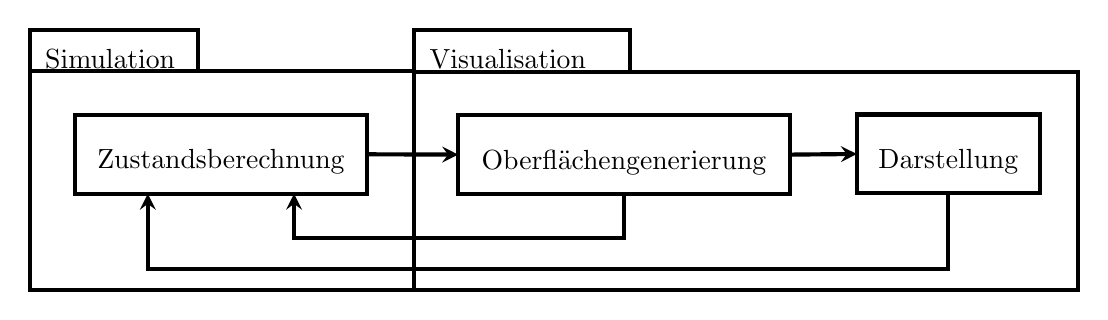
\begin{tikzpicture}
\pgftransformxscale{1.000000}
\pgftransformyscale{-1.000000}
\definecolor{dialinecolor}{rgb}{0.000000, 0.000000, 0.000000}
\pgfsetstrokecolor{dialinecolor}
\definecolor{dialinecolor}{rgb}{1.000000, 1.000000, 1.000000}
\pgfsetfillcolor{dialinecolor}
\pgfsetlinewidth{0.100000\du}
\pgfsetdash{}{0pt}
\definecolor{dialinecolor}{rgb}{1.000000, 1.000000, 1.000000}
\pgfsetfillcolor{dialinecolor}
\fill (25.450000\du,15.700000\du)--(25.450000\du,20.973357\du)--(34.750000\du,20.973357\du)--(34.750000\du,15.700000\du)--cycle;
\definecolor{dialinecolor}{rgb}{0.000000, 0.000000, 0.000000}
\pgfsetstrokecolor{dialinecolor}
\draw (25.450000\du,15.700000\du)--(25.450000\du,20.973357\du)--(34.750000\du,20.973357\du)--(34.750000\du,15.700000\du)--cycle;
\definecolor{dialinecolor}{rgb}{1.000000, 1.000000, 1.000000}
\pgfsetfillcolor{dialinecolor}
\fill (25.450000\du,14.700000\du)--(25.450000\du,15.700000\du)--(29.500000\du,15.700000\du)--(29.500000\du,14.700000\du)--cycle;
\definecolor{dialinecolor}{rgb}{0.000000, 0.000000, 0.000000}
\pgfsetstrokecolor{dialinecolor}
\draw (25.450000\du,14.700000\du)--(25.450000\du,15.700000\du)--(29.500000\du,15.700000\du)--(29.500000\du,14.700000\du)--cycle;
% setfont left to latex
\definecolor{dialinecolor}{rgb}{0.000000, 0.000000, 0.000000}
\pgfsetstrokecolor{dialinecolor}
\node[anchor=west] at (25.550000\du,15.400000\du){Simulation};
\definecolor{dialinecolor}{rgb}{1.000000, 1.000000, 1.000000}
\pgfsetfillcolor{dialinecolor}
\fill (26.532500\du,16.750000\du)--(26.532500\du,18.650000\du)--(33.577500\du,18.650000\du)--(33.577500\du,16.750000\du)--cycle;
\pgfsetlinewidth{0.100000\du}
\pgfsetdash{}{0pt}
\pgfsetdash{}{0pt}
\pgfsetmiterjoin
\definecolor{dialinecolor}{rgb}{0.000000, 0.000000, 0.000000}
\pgfsetstrokecolor{dialinecolor}
\draw (26.532500\du,16.750000\du)--(26.532500\du,18.650000\du)--(33.577500\du,18.650000\du)--(33.577500\du,16.750000\du)--cycle;
% setfont left to latex
\definecolor{dialinecolor}{rgb}{0.000000, 0.000000, 0.000000}
\pgfsetstrokecolor{dialinecolor}
\node at (30.055000\du,17.887500\du){Zustandsberechnung};
\pgfsetlinewidth{0.100000\du}
\pgfsetdash{}{0pt}
\definecolor{dialinecolor}{rgb}{1.000000, 1.000000, 1.000000}
\pgfsetfillcolor{dialinecolor}
\fill (34.710000\du,15.707955\du)--(34.710000\du,20.973357\du)--(50.705692\du,20.973357\du)--(50.705692\du,15.707955\du)--cycle;
\definecolor{dialinecolor}{rgb}{0.000000, 0.000000, 0.000000}
\pgfsetstrokecolor{dialinecolor}
\draw (34.710000\du,15.707955\du)--(34.710000\du,20.973357\du)--(50.705692\du,20.973357\du)--(50.705692\du,15.707955\du)--cycle;
\definecolor{dialinecolor}{rgb}{1.000000, 1.000000, 1.000000}
\pgfsetfillcolor{dialinecolor}
\fill (34.710000\du,14.707955\du)--(34.710000\du,15.707955\du)--(39.915000\du,15.707955\du)--(39.915000\du,14.707955\du)--cycle;
\definecolor{dialinecolor}{rgb}{0.000000, 0.000000, 0.000000}
\pgfsetstrokecolor{dialinecolor}
\draw (34.710000\du,14.707955\du)--(34.710000\du,15.707955\du)--(39.915000\du,15.707955\du)--(39.915000\du,14.707955\du)--cycle;
% setfont left to latex
\definecolor{dialinecolor}{rgb}{0.000000, 0.000000, 0.000000}
\pgfsetstrokecolor{dialinecolor}
\node[anchor=west] at (34.810000\du,15.407955\du){Visualisation};
\definecolor{dialinecolor}{rgb}{1.000000, 1.000000, 1.000000}
\pgfsetfillcolor{dialinecolor}
\fill (35.770708\du,16.757816\du)--(35.770708\du,18.657816\du)--(43.755708\du,18.657816\du)--(43.755708\du,16.757816\du)--cycle;
\pgfsetlinewidth{0.100000\du}
\pgfsetdash{}{0pt}
\pgfsetdash{}{0pt}
\pgfsetmiterjoin
\definecolor{dialinecolor}{rgb}{0.000000, 0.000000, 0.000000}
\pgfsetstrokecolor{dialinecolor}
\draw (35.770708\du,16.757816\du)--(35.770708\du,18.657816\du)--(43.755708\du,18.657816\du)--(43.755708\du,16.757816\du)--cycle;
% setfont left to latex
\definecolor{dialinecolor}{rgb}{0.000000, 0.000000, 0.000000}
\pgfsetstrokecolor{dialinecolor}
\node at (39.763208\du,17.895316\du){Oberflächengenerierung};
\definecolor{dialinecolor}{rgb}{1.000000, 1.000000, 1.000000}
\pgfsetfillcolor{dialinecolor}
\fill (45.374312\du,16.742529\du)--(45.374312\du,18.642529\du)--(49.781812\du,18.642529\du)--(49.781812\du,16.742529\du)--cycle;
\pgfsetlinewidth{0.100000\du}
\pgfsetdash{}{0pt}
\pgfsetdash{}{0pt}
\pgfsetmiterjoin
\definecolor{dialinecolor}{rgb}{0.000000, 0.000000, 0.000000}
\pgfsetstrokecolor{dialinecolor}
\draw (45.374312\du,16.742529\du)--(45.374312\du,18.642529\du)--(49.781812\du,18.642529\du)--(49.781812\du,16.742529\du)--cycle;
% setfont left to latex
\definecolor{dialinecolor}{rgb}{0.000000, 0.000000, 0.000000}
\pgfsetstrokecolor{dialinecolor}
\node at (47.578062\du,17.880029\du){Darstellung};
\pgfsetlinewidth{0.100000\du}
\pgfsetdash{}{0pt}
\pgfsetdash{}{0pt}
\pgfsetbuttcap
{
\definecolor{dialinecolor}{rgb}{0.000000, 0.000000, 0.000000}
\pgfsetfillcolor{dialinecolor}
% was here!!!
\pgfsetarrowsend{stealth}
\definecolor{dialinecolor}{rgb}{0.000000, 0.000000, 0.000000}
\pgfsetstrokecolor{dialinecolor}
\draw (33.577500\du,17.700000\du)--(35.770708\du,17.707816\du);
}
\pgfsetlinewidth{0.100000\du}
\pgfsetdash{}{0pt}
\pgfsetdash{}{0pt}
\pgfsetbuttcap
{
\definecolor{dialinecolor}{rgb}{0.000000, 0.000000, 0.000000}
\pgfsetfillcolor{dialinecolor}
% was here!!!
\pgfsetarrowsend{stealth}
\definecolor{dialinecolor}{rgb}{0.000000, 0.000000, 0.000000}
\pgfsetstrokecolor{dialinecolor}
\draw (43.755708\du,17.707816\du)--(45.374312\du,17.692529\du);
}
\pgfsetlinewidth{0.100000\du}
\pgfsetdash{}{0pt}
\pgfsetdash{}{0pt}
\pgfsetmiterjoin
\pgfsetbuttcap
{
\definecolor{dialinecolor}{rgb}{0.000000, 0.000000, 0.000000}
\pgfsetfillcolor{dialinecolor}
% was here!!!
\pgfsetarrowsend{stealth}
{\pgfsetcornersarced{\pgfpoint{0.000000\du}{0.000000\du}}\definecolor{dialinecolor}{rgb}{0.000000, 0.000000, 0.000000}
\pgfsetstrokecolor{dialinecolor}
\draw (39.763208\du,18.657816\du)--(39.763208\du,19.707816\du)--(31.816250\du,19.707816\du)--(31.816250\du,18.650000\du);
}}
\pgfsetlinewidth{0.100000\du}
\pgfsetdash{}{0pt}
\pgfsetdash{}{0pt}
\pgfsetmiterjoin
\pgfsetbuttcap
{
\definecolor{dialinecolor}{rgb}{0.000000, 0.000000, 0.000000}
\pgfsetfillcolor{dialinecolor}
% was here!!!
\pgfsetarrowsend{stealth}
{\pgfsetcornersarced{\pgfpoint{0.000000\du}{0.000000\du}}\definecolor{dialinecolor}{rgb}{0.000000, 0.000000, 0.000000}
\pgfsetstrokecolor{dialinecolor}
\draw (47.578062\du,18.642529\du)--(47.578062\du,20.468821\du)--(28.293750\du,20.468821\du)--(28.293750\du,18.650000\du);
}}
\end{tikzpicture}

  \caption{Vereinfachte Programmstruktur}
  \label{fig:programmstruktur}
\end{figure}
Lässt man das Host-Programm außer Acht, da es neben den Metafunktionalitäten Initialisierung und Organisation keine substanziellen Funktionen zu der Wassersimulation beiträgt, besteht das Programm also aus den drei Teilen \textit{Zustandsberechnung}, \textit{Oberflächengenerierung} und \textit{Darstellung}. \\
Sowohl die Zustandsberechnung als auch die Oberflächengenerierung wurden mithilfe von OpenCL implementiert und werden, da die entsprechenden Kernel in dieselbe geordnete Warteschlange eingereiht werden, streng sequentiell ausgeführt. Die Darstellung hingegen wurde mithilfe von OpenGL umgesetzt und wird tendenziell jeweils nach den OpenCL-Berechnungen ausgeführt, allerdings wird dieses Verhalten nicht vom Host-Programm forciert.\\
Getreu der dargestellten Trennung wird im weiteren Verlauf dieser Ausarbeitung in Kapitel~\ref{chap:sph} auf die Simulation und in Kapitel~\ref{chap:visualisierung} auf die Visualisierung näher eingegangen.